\documentclass[tikz]{standalone}
\usetikzlibrary{positioning,arrows.meta}

\begin{document}
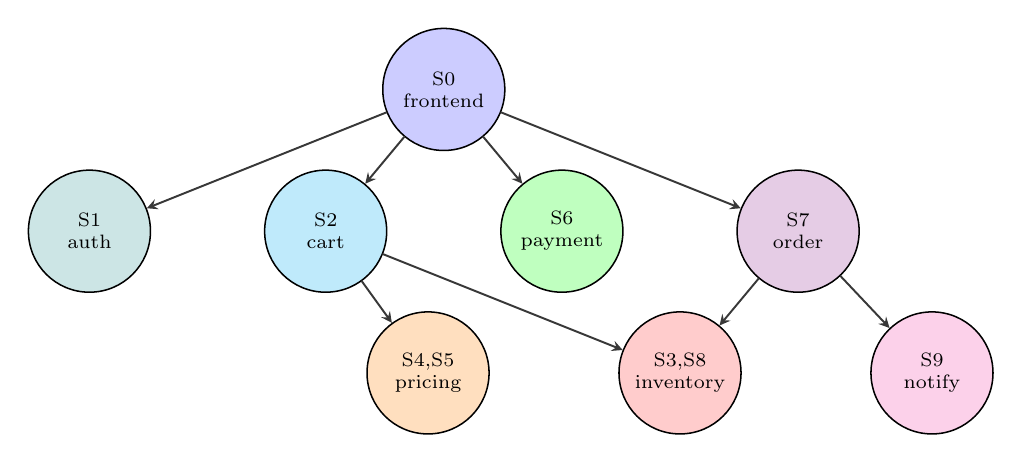
\begin{tikzpicture}[
  service/.style={draw, circle, minimum size=1.55cm, align=center, font=\scriptsize, inner sep=1pt, line width=0.55pt},
  edge/.style={->, >=stealth, line width=0.7pt, black!78, line cap=round}
]

% Layered placement by logical depth from waterfall call structure.
% Depth 0
\node[service, fill=blue!20] (s0) at (0,4.4) {S0\\frontend};

% Depth 1
\node[service, fill=teal!20] (s1) at (-4.5,2.6) {S1\\auth};
\node[service, fill=cyan!25] (s2) at (-1.5,2.6) {S2\\cart};
\node[service, fill=green!25] (s6) at (1.5,2.6) {S6\\payment};
\node[service, fill=violet!20] (s7) at (4.5,2.6) {S7\\order};

% Depth 2
\node[service, fill=orange!25] (s45) at (-0.2,0.8) {S4,S5\\pricing};
\node[service, fill=red!20] (s38) at (3.0,0.8) {S3,S8\\inventory};
\node[service, fill=magenta!18] (s9) at (6.2,0.8) {S9\\notify};

% Straight edges only
\draw[edge] (s0) -- (s1);
\draw[edge] (s0) -- (s2);
\draw[edge] (s0) -- (s6);
\draw[edge] (s0) -- (s7);
\draw[edge] (s2) -- (s45);
\draw[edge] (s2) -- (s38);
\draw[edge] (s7) -- (s38);
\draw[edge] (s7) -- (s9);


\end{tikzpicture}
\end{document}
